\documentclass{article}
\usepackage{float}
\usepackage{hyperref}
\usepackage[utf8]{inputenc}
\usepackage{graphicx}
\usepackage{caption}
\usepackage{subcaption}
\usepackage{algpseudocode}
\usepackage{algorithm}
\usepackage{mathtools}
\usepackage{amsmath,amssymb}
\usepackage{siunitx}
\usepackage{listings}
\usepackage{bbm}
\usepackage[most]{tcolorbox}
\newcommand{\e}[1]{{\mathbb E}\left[ #1 \right]}
\definecolor{block-gray}{gray}{0.90}
\newtcolorbox{code}{colback=block-gray,grow to right by=-1mm,grow to left by=-1mm,boxrule=0pt,boxsep=0pt,breakable}
\lstset{
  basicstyle=\ttfamily,
  columns=fullflexible,
  frame=single,
  breaklines=true,
  postbreak=\mbox{\textcolor{red}{$\hookrightarrow$}\space},
}

\title{\vspace{-3cm}Charlie meeting 30th May\vspace{-3em}}
\author{}
\date{}

\begin{document}
\maketitle
This meeting we start implementing some ideas. 
We have two main sources of information, trajectory and invariances. 
We will see if there is a  difference between conditioning on invariances or not.
We model $v(\mathbf{x}) \text{and} a(\mathbf{x})$ as two independent GP prior, with kernel $K_v, K_a$.
We denote $X_g$ as the grid points of invariances conditioning, $X^{*}$ as our test points and $X$ as our trajectory data. 
Since the invariance of a simple harmonic oscillator is conservation of energy, $\dot{x}a+xv=0$
We will have 
$$
  \begin{multlined}
    \begin{pmatrix}
      v(X)\\
      v(X^*)\\
      a(X)\\
      a(X^*)\\
      \dot{x}_ga(X_g)+x_gv(X_g)
    \end{pmatrix}
    \sim \mathcal{N}
    \left(
    \begin{pmatrix}
      0\\0\\0\\0\\0
    \end{pmatrix}
    ,\\
    \begin{pmatrix}
      K_v(X,X)+\sigma^2\mathcal{I} & K_v(X, X^*) & 0 & 0 & x_g*K_v(X, X_g)\\
      K_v(X^*, X) & K_v(X^*, X^*) & 0 & 0 & x_g*K_v(X^*,X_g)\\
      0 & 0 & K_a(X, X)+\sigma^2\mathcal{I} & K_a(X, X^*) & \dot{x}_g*K_a(X, X_g)\\
      0 & 0 & K_a(X^*,X) & K_a(X^*, X^*) & \dot{x}_g*K_a(X^*, X_g)\\
      x_g*K_v(X_g, X) & x_g*K_v(X_g, X^*) & \dot{x}_g*K_a(X_g, X) & \dot{x}_g*K_a(X_g, X^*) & \dot{x}_g*K_a(X_g, X_g)*\dot{x}_g^T + x_g*K_v(X_g, X_g)*x_g^T\\
    \end{pmatrix}
    \right)
  \end{multlined}
$$
Here, $*$ means element wise multiplication
Using the Gaussian condtional formula again
$$
\begin{aligned}
p\left(\left[\begin{array}{l}
\mathbf{x}_{1} \\
\mathbf{x}_{2}
\end{array}\right]\right) &=\mathcal{N}\left(\left[\begin{array}{l}
\mathbf{x}_{1} \\
\mathbf{x}_{2}
\end{array}\right] ;\left[\begin{array}{l}
\boldsymbol{\mu}_{1} \\
\boldsymbol{\mu}_{2}
\end{array}\right],\left[\begin{array}{ll}
\boldsymbol{\Sigma}_{11} & \boldsymbol{\Sigma}_{12} \\
\boldsymbol{\Sigma}_{21} & \boldsymbol{\Sigma}_{22}
\end{array}\right]\right) \\
p\left(\mathbf{x}_{1} \mid \mathbf{x}_{2}\right) &=\mathcal{N}\left(\mathbf{x}_{1} ; \boldsymbol{\mu}_{1}+\boldsymbol{\Sigma}_{12} \Sigma_{22}^{-1}\left(\mathbf{x}_{2}-\boldsymbol{\mu}_{2}\right), \boldsymbol{\Sigma}_{11}-\boldsymbol{\Sigma}_{12} \boldsymbol{\Sigma}_{22}^{-1} \boldsymbol{\Sigma}_{21}\right)
\end{aligned}
$$
This time, for $v(X*)|v(X)=\mathcal{D}, a(X_g,\dot{X}_g)\dot{X}_g +v(X_g, \dot{X}_g)X_g=0$ 

we have $\Sigma_{11}=K_v(X^*, X^*), \Sigma_{12}=[K_v(X^*, X), x_g*K_v(X^*, X_g)], \Sigma_{21} = \begin{bmatrix}
  K_v(X, X^*)\\x_g*K_v(X_g, X^*)
\end{bmatrix}, \Sigma_{22}=\begin{bmatrix}
  K_v(X, X)+\sigma^2\mathcal{I} & x_g*K_v(X,X_g) \\ x_g*K_v(X_g, X) & \dot{x}_g*K_a(X_g, X_g)*\dot{x}_g^T + x_g*K_v(X_g, X_g)*x_g^T
\end{bmatrix}$, 

Therefore, we have 
$$
p(v(X^*)|v(X)=\mathcal{D},a(X_g,\dot{X}_g)*\dot{x}_g +v(X_g, \dot{X}_g)*x_g=0)\sim\mathcal{N}\left(\Sigma_{12}\Sigma_{22}^{-1}\begin{bmatrix}
  \mathcal{D}\\0
\end{bmatrix}, \Sigma_{11}-\Sigma_{12}\Sigma_{22}^{-1}\Sigma_{21}\right)
$$

Similarly, for acceleartion, 
 $a(X*)|a(X)=\mathcal{D}, a(X_g,\dot{X}_g)\dot{X}_g +v(X_g, \dot{X}_g)X_g=0$ 

we have $\Sigma_{11}=K_a(X^*, X^*)$, 
$\Sigma_{12}=[K_a(X^*, X), \dot{x}_g*K_a(X^*, X_g)]$, 
$\Sigma_{21} = \begin{bmatrix}
  K_a(X, X^*)\\\dot{x}_g*K_a(X_g, X^*)
\end{bmatrix}$,
$\Sigma_{22}=\begin{bmatrix}
  K_a(X, X)+\sigma^2\mathcal{I} & \dot{x}_g*K_a(X,X_g) \\ \dot{x}_g*K_a(X_g, X) & \dot{x}_g*K_a(X_g, X_g)*\dot{x}_g^T + x_g*K_v(X_g, X_g)*x_g^T
\end{bmatrix}$, 

which has mean
$$
[K_a(X^*, X), \dot{x}_g*K_a(X^*, X_g)]\begin{bmatrix}
  K_a(X, X)+\sigma^2\mathcal{I} & \dot{x}_g*K_a(X,X_g) \\ \dot{x}_g*K_a(X_g, X) & \dot{x}_g*K_a(X_g, X_g)*\dot{x}_g^T + x_g*K_v(X_g, X_g)*x_g^T
\end{bmatrix}^{-1}\begin{bmatrix}\mathcal{D}\\0\end{bmatrix}$$
and covariance
$$
  \begin{multlined}
K_a(X^*,X^*)-\\\left[K_a(X^*, X), \dot{x}_g*K_a(X^*, X_g)\right]\begin{bmatrix}
  K_a(X, X)+\sigma^2\mathcal{I} & \dot{x}_g*K_a(X,X_g) \\ \dot{x}_g*K_a(X_g, X) & \dot{x}_g*K_a(X_g, X_g)*\dot{x}_g^T + x_g*K_v(X_g, X_g)*x_g^T
\end{bmatrix}^{-1} \begin{bmatrix}
  K_a(X, X^*)\\\dot{x}_g*K_a(X_g, X^*)
\end{bmatrix}\begin{bmatrix}
  K_a(X, X)+\sigma^2\mathcal{I} & \dot{x}_g*K_a(X,X_g) \\ \dot{x}_g*K_a(X_g, X) & \dot{x}_g*K_a(X_g, X_g)*\dot{x}_g^T + x_g*K_v(X_g, X_g)*x_g^T
\end{bmatrix}
\end{multlined}
$$

I mainly just showed the results for acceleration from now onwards since vecloity is pretty much the same as we model them as independent.
I performed the computation manually (manually invert matrix and do matrix multiplication) because I don't know how to fit it into GPflow.
I first used a grid as invaraince points.
My data is simulated by just a simple sine curve for position and cosine curve for velocity. I then took the finite time difference to find the acceleartion and vecloity as targets.
I took 20 by 20 invarince points from -5 to 5.
I have also calculate the invariance prior conditioning the test points just on the invariance but not the trajectory data.
The result is as follows (this is for the highest marginal likelihood, length scale 1, likelihood variance 0.01, and invariance density 10):
The first two are normal GPs, the blackdots are the data and the grey surface is the uncertainity. 
For contours, the ring in the middle is the data. 
The last four are invariance GPs (prior and posterior), and the red dots are where I put the conditioning invariance points.
\begin{figure}[H]
  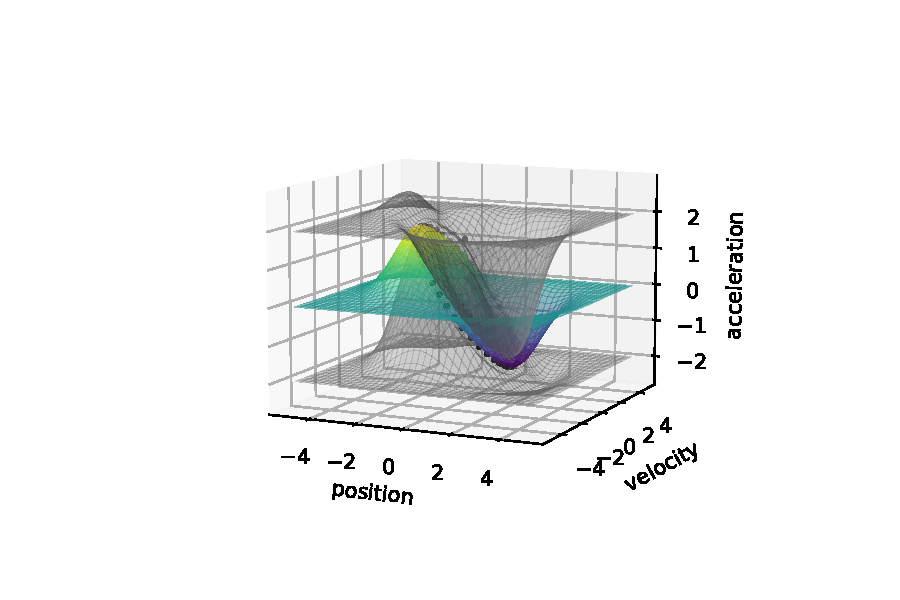
\includegraphics[width=1.2\linewidth]{regular_3D.pdf}
  \centering
\end{figure}
\begin{figure}[H]
  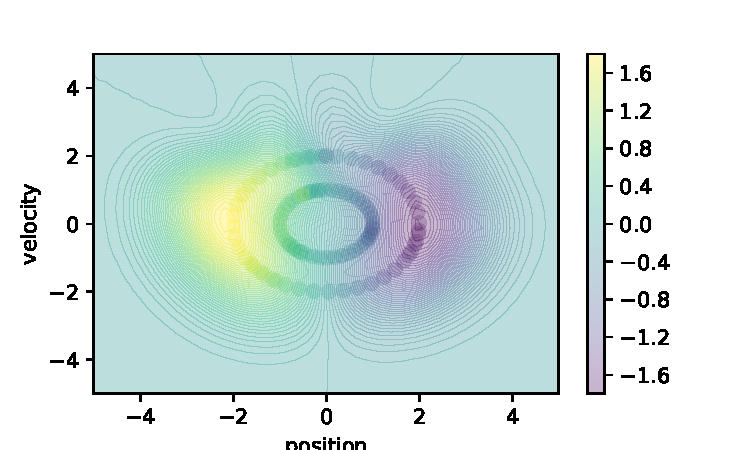
\includegraphics[width=\linewidth]{regular_contour.pdf}
  \centering
\end{figure}
\begin{figure}[H]
  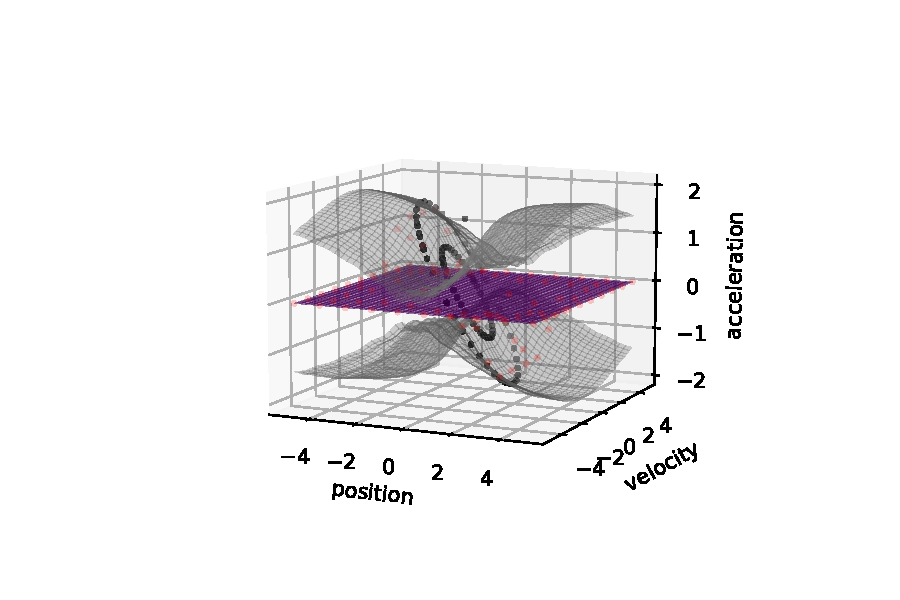
\includegraphics[width=1.2\linewidth]{prior_invariance_3D.pdf}
  \centering
\end{figure}
\begin{figure}[H]
  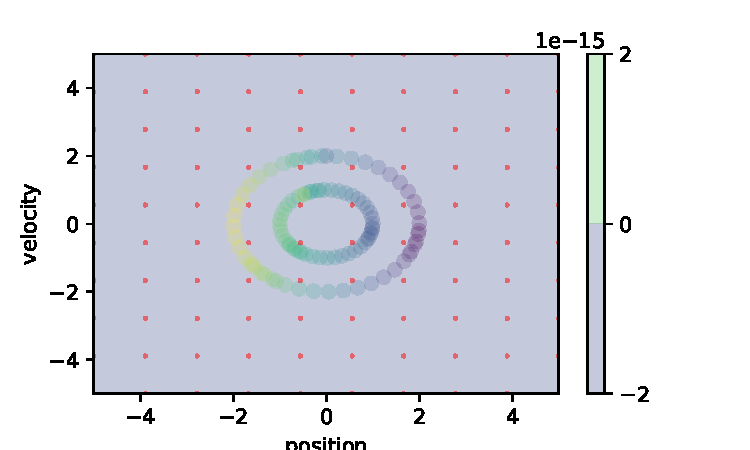
\includegraphics[width=\linewidth]{prior_invariance_contour.pdf}
  \centering
\end{figure}
\begin{figure}[H]
  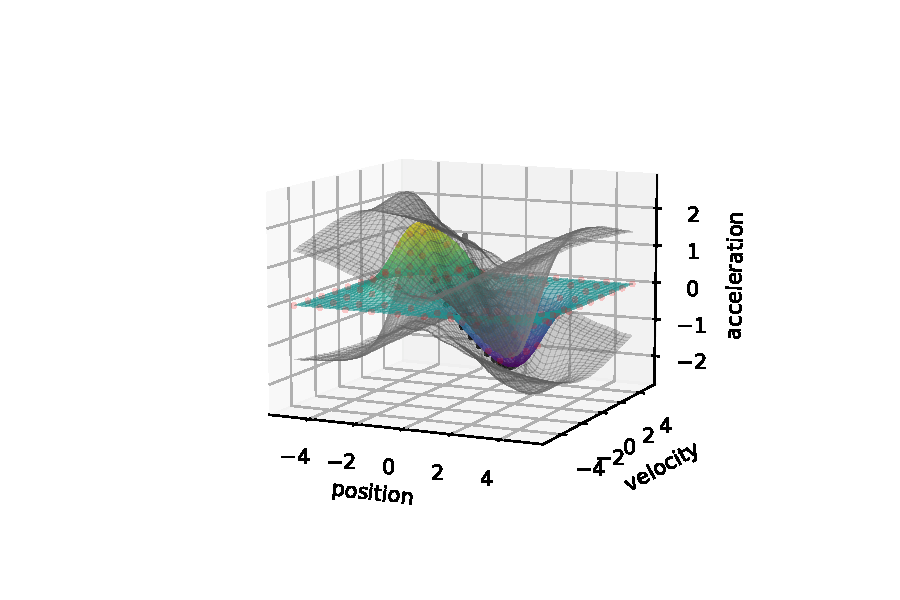
\includegraphics[width=1.2\linewidth]{posterior_invariance_3D.pdf}
  \centering
\end{figure}
\begin{figure}[H]
  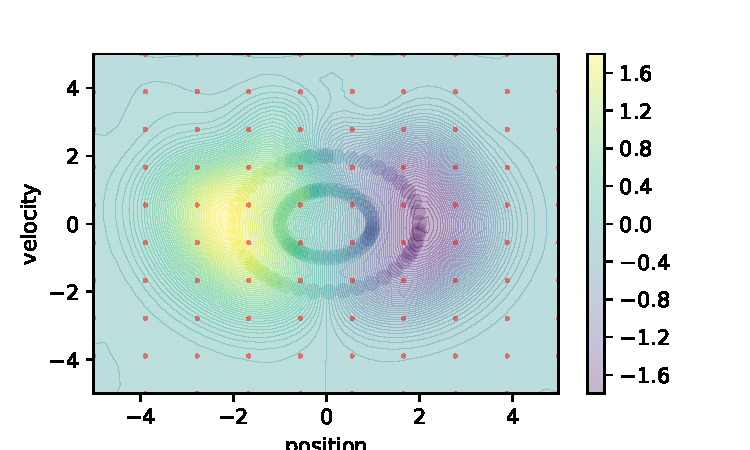
\includegraphics[width=\linewidth]{posterior_invariance_contour.pdf}
  \centering
\end{figure}

It does not seem to change the mean function, but the variance seems to have reduced, is that a positive result?
The analytical solution of acceleration should be equal to $-x$ so we should have a flat plane in the $-45$ degrees direction. 
I calculated the marginal likelihood as below, please check if the calculation is correct. 
I have tried increase the density of invariance and the result varied accordingly, so I suppose this is a "hyperparamter" to tune too.

In all cases, when the invariance kernel is valid, (determinant $\ge0$), the invariance performace are almost all better than the regular version.

The log marginal likelihood is worked out to be 
$$
\begin{aligned}
p(y|X,\theta) &= \int p(y|f, X)p(f_{inv}|X, \theta)df\\ &= \int \mathcal{N}(y|f, \sigma^2I)p(f(X)|\text{invaraince}, \theta)df\\ &= \int \mathcal{N}(y|f, \sigma^2I)\mathcal{N}(f_{inv}|0,K(X, X)-x_g*K(X, X_g)[\dot{x}_gK_a\dot{x}_g^T+x_gK_vx_g^T]^{-1}x_g*K(X_g, X))\\
&=\mathcal{N}(y|0, \sigma^2I+K(X, X)-x_g*K(X, X_g)[\dot{x}_gK_a\dot{x}_g^T+x_gK_vx_g^T]^{-1}x_g*K(X_g, X))
\end{aligned}
$$
Therefore, the log marginal likelihood will be
$$
\log p(\boldsymbol{y} \mid \boldsymbol{X}, \boldsymbol{\theta})=-\frac{1}{2} \boldsymbol{y}^{\top} \boldsymbol{K}_{\boldsymbol{\theta}}^{-1} \boldsymbol{y}-\frac{1}{2} \log \left|\boldsymbol{K}_{\boldsymbol{\theta}}\right|+\text { const }
$$, where $K_\theta$ will be the covariance derived in the previous equation.
Therefore, we note that the grid of invariance is also a hyperparamter to be integrated over.

When I am changing my parameters, sometimes the marginal likelihood would be not defined due to the determinant of the kernel being negative, which shouldn't be if it is a valid covaraince matrix. 
So how do we to make sure the new kernel is still positive definite or a valid covariance matrix?


To implement the kernel in GPflow, I need to find the covariance of two matrix X, X1 and X2, condition on the invaraince in closed form.
This will require me to find the joint distribution of X1, X2 condition on the invariance; therefore this time, I will need to find the covariance function between X1 and X2 and conditioning.
I have 
$$
\begin{pmatrix}
  f(X1)  \\ f(X2)
\end{pmatrix}|\text{invariance}
\sim \mathcal{N}
\left(
\begin{pmatrix}
  0\\0
\end{pmatrix}  
,
\begin{pmatrix}
K_{inv}(X1, X1) & K_{inv}(X1, X2) \\ K_{inv}(X2, X1) & K_{inv}(X2, X2)  
\end{pmatrix}
\right)
$$
At the same time, we have the normal condition formula as before
with the covariance equal to 
$$
\begin{multlined}
\begin{bmatrix}
  K_a(X1, X1) & K_a(X1, X2) \\ K_a(X2, X1) & K_a(X2, X2)\\
\end{bmatrix}
-\\
\begin{bmatrix}
  \dot{x}_g*K_a(X1, X_g) \\ \dot{x}_g*K_a(X2, X_g)
\end{bmatrix}
\left[\dot{x}_g*K_a(X_g, X_g)*\dot{X}_g^T+x_g*K_v(X_g, X_g)*X_g^T\right]^{-1}\left[\dot{x}_g*K_a(X1, X_g), \dot{x}_g*K_a(X2, X_g)\right]
\end{multlined}
$$

and similarly for vecloity, I am actually not sure if we can write it as a general kernel, since after I condition the joint distribution of X1, X2 on invariance, I will get something that I am not sure how to put it into the closed form.

\section*{To discuss}
\begin{enumerate}
  \item is it a good result?
  \item is it possible to extend it to the whole phase space
  \item how to write the invariance kernel analytically
  \item what's the next step
\end{enumerate}


\end{document}

